\documentclass[]{slides}
\title{Low-power design techniques}

% Begin document
\begin{document}
%\printpdftrue % uncomment to hide pauses
% Title slide
\begin{frame} \titlepage \end{frame}

% Outline slide
%\begin{frame}{Outline} \tableofcontents \end{frame}

% ====================
% Low-power design techniques
% ====================
\begin{frame}{Power in ICs}{}
\alertblue{Definitions}
\begin{itemize}
\item \alertblue{Dynamic power}. Power dissipated in \acp{IC} due to switching activity.
\begin{itemize}
  \item Charging and discharging load capacitances.
  \item Short-circuit current, when both pMOS and nMOS transistors are on for a brief period.
\end{itemize}
\item \alertblue{Static power}. Power dissipated in \acp{IC} even when there is no switching activity.
\begin{itemize}
  \item Gate and junction leakages.
\end{itemize}
\end{itemize}
\end{frame}

% ====================
% Dynamic power
% ====================
\begin{frame}{Dynamic power}{}
\alertblue{Dynamic power}
\begin{itemize}
\item Dynamic power is described in \eref{eq:DynamicPower}
\begin{equation}
\label{eq:DynamicPower}
P_{dyn} = \alpha C_{L} V_{DD}^{2} f_{clk}
\end{equation} 
\item[]where
\item[]$\alpha \in [0,1]$ is a switching activity factor respect to a clock source, \ie, clock signals have $\alpha=1$. It determines the probability of a net transitioning from 0 to 1,
\item[]$C_{L}$ is the capacitive load,
\item[]$V_{DD}^{2}$ is the supply voltage,
\item[]$f_{clk}$ is the clock frequency.
\end{itemize}
\end{frame}

% ====================
% Low-power techniques
% ====================
\begin{frame}{Low-power design techniques}{}
\alertblue{Low-power design techniques}
\begin{itemize}
\item \alertblue{\ac{DVFS}} for reducing dynamic power.
\item \alertblue{Clock gating} for reducing dynamic power .
\item \alertblue{Power gating} for reducing static power.
\end{itemize}
\end{frame}

\section{Dynamic Voltage and Frequency Scaling}
% ====================
% DVFS
% ====================
\begin{frame}{Low-power design techniques}{}
\alertblue{\acl{DVFS}}
\begin{itemize}
\item From \eref{eq:DynamicPower}, we can see that the supply voltage has a quadratic effect on power dissipation.
\begin{equation*}
P_{dyn} = \alpha C_{L} V_{DD}^{2} f_{clk}
\end{equation*}
\item[]As a result, we may simply lower $V_{DD}$.
\item Example: What is the power saving in a system that reduces $V_{DD}$ from 1~V to 0.85~V?
\pause
\begin{equation*}
\frac{P_{dyn2}}{P_{dyn1}} = \frac{\alpha C_{L} \cdot 0.85^{2} \cdot f_{clk}}{\alpha C_{L} \cdot 1^{2} \cdot f_{clk}} = 0.7225
\end{equation*}
In other words,
\begin{equation*}
P_{dyn2}= 0.7225 \times P_{dyn1} 
\end{equation*}
\end{itemize}
\end{frame}

% ====================
% DVFS
% ====================
\begin{frame}{Low-power design techniques}{}
\alertblue{\acl{DVFS}}
\begin{itemize}
\item In the previous example, we are reducing power consumption by 27.75\% by reducing only 15\% of the power supply.
\item However, we can't simply reduce $V_{DD}$ without consequences.
\pause
\item Propagation delays in \acf{CMOS} transistors are an inversely proportional function of $V_{DD}$.
\begin{itemize}
  \item Larger $V_{DD}$ values yield smaller propagation delays.
\end{itemize}
\item As a result of this, $f_{clk}$ must be adapted.
\end{itemize}
\end{frame}

% ====================
% DVFS
% ====================
\begin{frame}{Low-power design techniques}{}
\alertblue{\acl{DVFS}}
\begin{itemize}
\item \ac{DVFS} consists of modifying both $V_{DD}$ and $f_{clk}$ according to the processing and power requirements of the system.
\end{itemize}
\begin{figure}
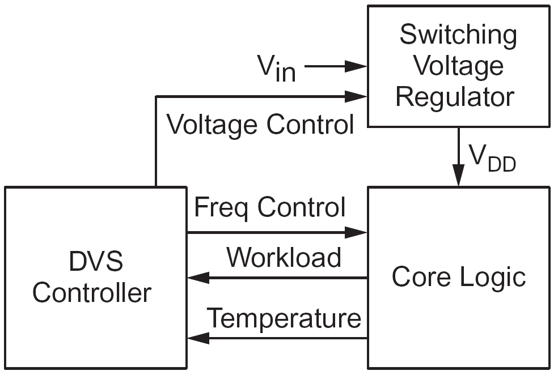
\includegraphics[scale=0.3]{LowPower_DVFS_block}
\caption{DVFS basic block diagram.}
\label{Figure:DVFS_block}
\end{figure}

\end{frame}

% ====================
% DVFS
% ====================
\begin{frame}{Low-power design techniques}{}
\alertblue{\acl{DVFS}}
\begin{itemize}
\item Voltage and frequency pairs are usually stored inside the \ac{DVFS} controller.
\item These values may be pre-loaded or may be calculated on-the-fly using performance statistics through performance evaluation algorithms.
\end{itemize}
\end{frame}

\section{Clock Gating}
% ====================
% Clock gating
% ====================
\begin{frame}{Low-power design techniques}{}
\alertblue{Clock gating}
\begin{itemize}
\item Another factor that can be easily modified in \eref{eq:DynamicPower} is the switching activity $\alpha$.
\begin{equation*}
P_{dyn} = \alpha C_{L} V_{DD}^{2} f_{clk}
\end{equation*}
\item This may be achieved at the algorithmic level or at the \ac{RTL} level.
\item From the circuit point of view, we can disable the clock signal in certain blocks within the \ac{IC} that are idle.\\
\item This prevents any switching activity  and prevents and dynamic power dissipation.
\end{itemize}
\end{frame}

% ====================
% Clock gating
% ====================
\begin{frame}{Low-power design techniques}{}
\alertblue{Clock gating}
\begin{itemize}
\item Another factor that can be easily modified in \eref{eq:DynamicPower} is the switching activity $\alpha$.
\begin{equation*}
P_{dyn} = \alpha C_{L} V_{DD}^{2} f_{clk}
\end{equation*}
\item This may be achieved at the algorithmic level or at the \ac{RTL} level.
\item From the circuit point of view, we can disable the clock signal in certain blocks within the \ac{IC} that are idle.\\
\item This prevents any switching activity  and prevents and dynamic power dissipation.
\end{itemize}
\end{frame}

% ====================
% Clock gating
% ====================
\begin{frame}{Low-power design techniques}{}
\vspace{-5pt}
\alertblue{Clock gating}
\begin{figure}
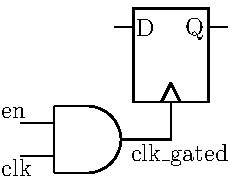
\includegraphics[scale=1]{LowPower_CG1}
\end{figure}
\vspace{-15pt}
\begin{figure}
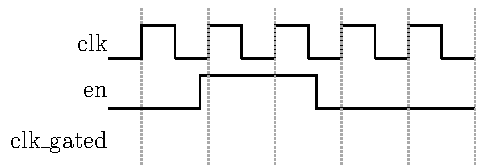
\includegraphics[width=0.9\textwidth]{LowPower_CG1_wave}
\end{figure}
\end{frame}

% ====================
% Clock gating
% ====================
\begin{frame}{Low-power design techniques}{}
\vspace{-5pt}
\alertblue{Clock gating}
\begin{figure}
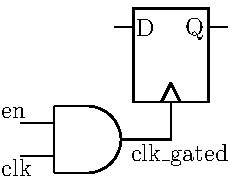
\includegraphics[scale=1]{LowPower_CG1}
\end{figure}
\vspace{-15pt}
\begin{figure}
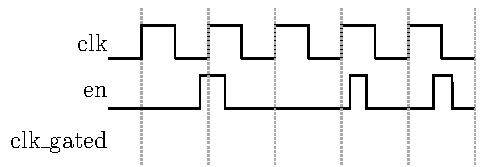
\includegraphics[width=0.9\textwidth]{LowPower_CG1_waveb}
\end{figure}
\end{frame}

% ====================
% Clock gating
% ====================
\begin{frame}{Low-power design techniques}{}
\vspace{-5pt}
\alertblue{Clock gating}
\begin{figure}
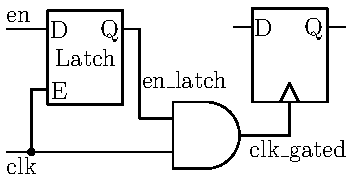
\includegraphics[scale=1]{LowPower_CG2}
\end{figure}
\vspace{-10pt}
\begin{figure}
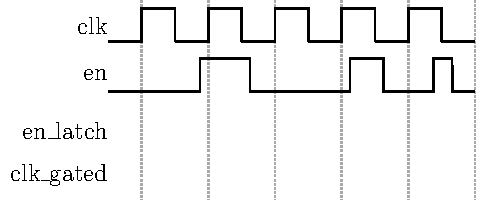
\includegraphics[width=0.85\textwidth]{LowPower_CG2_wave}
\end{figure}
\end{frame}

% ====================
% Clock gating
% ====================
\begin{frame}{Low-power design techniques}{}
\vspace{-5pt}
\alertblue{Clock gating}
\begin{figure}
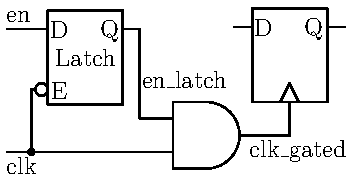
\includegraphics[scale=1]{LowPower_CG3}
\end{figure}
\vspace{-10pt}
\begin{figure}
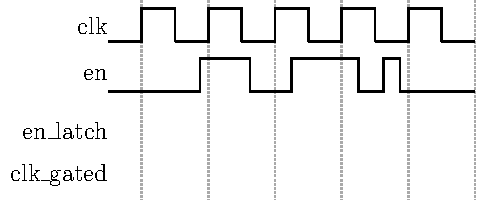
\includegraphics[width=0.85\textwidth]{LowPower_CG3_wave}
\end{figure}
\end{frame}

% ====================
% Clock gating
% ====================
\begin{frame}{Low-power design techniques}{}
\alertblue{Clock gating}
\begin{itemize}
\item Fortunately, designers don't have to connect latches, \code{AND} and flip-flops together every time they want to employ clock gating.
\item Standard cell libraries provide clock gating cells.
\end{itemize}
\begin{figure}
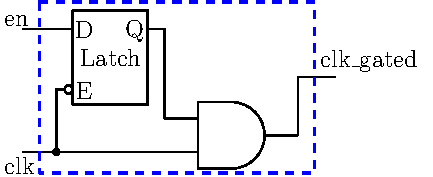
\includegraphics[scale=1]{LowPower_CG_cell}
\caption{Clock cell gate.}
\label{Figure:CG_cell}
\end{figure}
\begin{itemize}
\item Moreover, modern synthesizers are clever enough to detect and infer clock-gating cells when reading \ac{RTL}. 
\end{itemize}
\end{frame}

% ====================
% Clock gating
% ====================
\begin{frame}[fragile]{Low-power design techniques}{}
\alertblue{Clock gating}
\begin{itemize}
\item Clock gating may be easily implemented using a combination of \ac{RTL} coding style and synthesizer commands.
\end{itemize}
    \lstset{
    numbers=none,
    captionpos=t,
    title=Clock gating in RTL,
    xleftmargin=.2\textwidth, xrightmargin=.2\textwidth
  }
  \begin{lstlisting}
    always_ff @ (posedge clk)
        if(enable)
            Q <= D;
  \end{lstlisting}
  
\begin{itemize}
\item Synthesis tools such as Synopsys Design Compiler use commands such as
\begin{itemize}
  \item[] \code{set\_clock\_gating\_style -global -minimum\_bitwidth <value>}
\end{itemize}
 
\end{itemize}

\end{frame}

\section{Power Gating}
% ====================
% Power gating
% ====================
\begin{frame}{Low-power design techniques}{}
\alertblue{Power gating}
\begin{itemize}
\item Power gating consists on switching off entire parts of the \ac{IC} by temporarily disconnecting it from the supply rail.
\end{itemize}
\begin{figure}
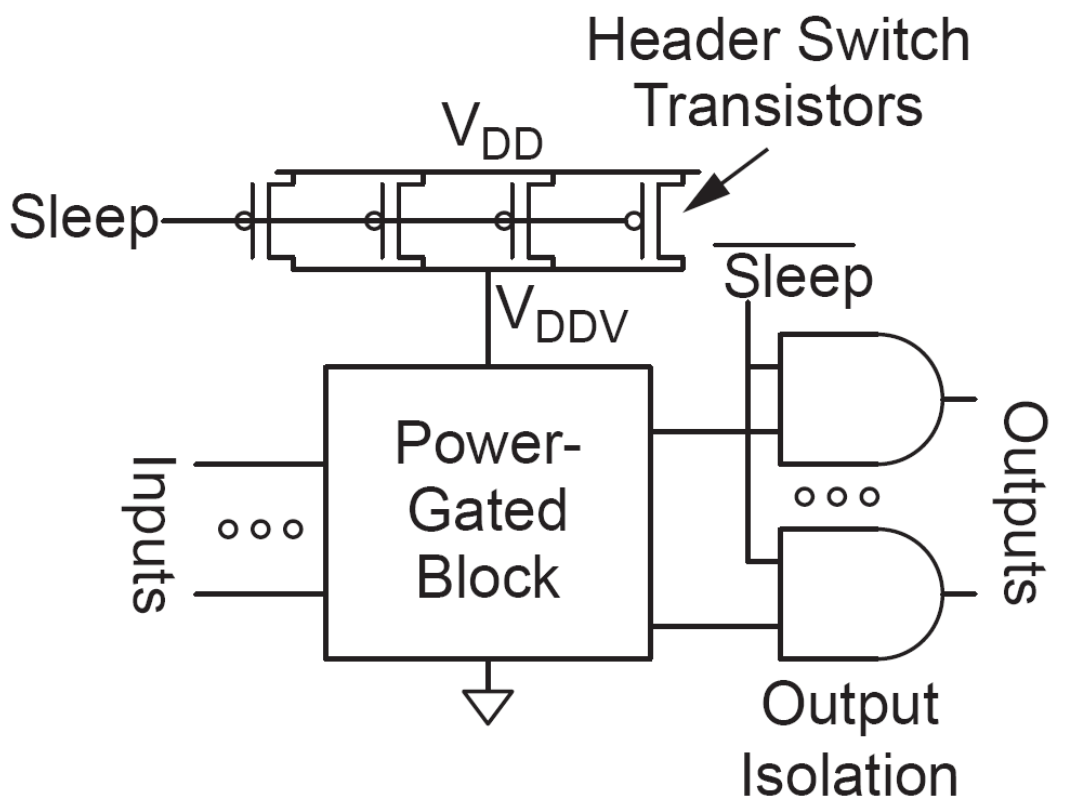
\includegraphics[scale=0.38]{LowPower_PG}
\caption{Power gating basic block diagram.}
\label{Figure:PG_block}
\end{figure}
\end{frame}

% ====================
% Power gating
% ====================
\begin{frame}{Low-power design techniques}{}
\alertblue{Power gating}
\begin{itemize}
\item Header switch  requires careful design.
\begin{itemize}
  \item Low leakage.
  \item Fast switching on times.
\end{itemize}
\item This technique is only efficient when blocks must be turned off for long periods.
\item When a block is turned off, its state must be saved in order to allow resuming execution.
\end{itemize}

\end{frame}
%% ====================
%% ISA vs uA
%% ====================
%\begin{frame}{\acl{ISA}}{Same \ac{ISA}, different \uA - 45~nm technology}
%\begin{figure}[!htb]
%  \begin{minipage}{0.5\textwidth}
%    \centering
%    \begin{itemize}
%      \item x86 \ac{ISA}.
%      \item Quad Core.
%      \item 2.6~GHz.
%      \item 125~W.
%    \end{itemize}
%    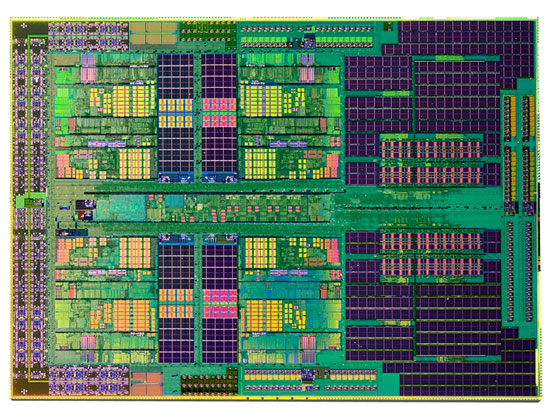
\includegraphics[width=0.8\linewidth]{ISA_AMD_Phenom_II_X4.jpg}
%    \caption{AMD Phenom X4}
%    \label{Figure:AMD_Phenom_X4a}
%  \end{minipage}%
%  \begin{minipage}{0.50\textwidth}
%    \centering
%    \begin{itemize}
%      \item x86 \ac{ISA}.
%      \item Dual Core.
%      \item 1.6~GHz.
%      \item 2~W.
%    \end{itemize}
%    \vspace{14mm}
%    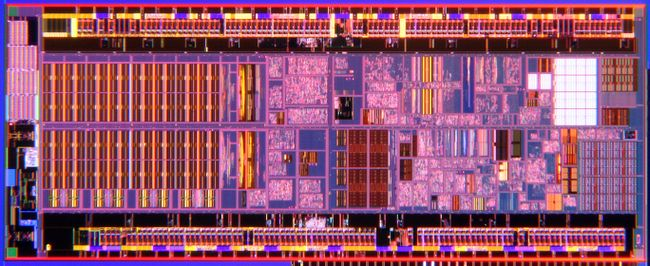
\includegraphics[width=0.92\linewidth]{ISA_Intel_Atom.jpg}
%    \caption{Intel Atom}
%    \label{Figure:Intel_Atom}
%  \end{minipage}
%\end{figure}
%\end{frame}




%% ====================
%% ISA characteristics: Registers
%% ====================
%\begin{frame}{Basic registers of a computer}{}
%\begin{figure}
%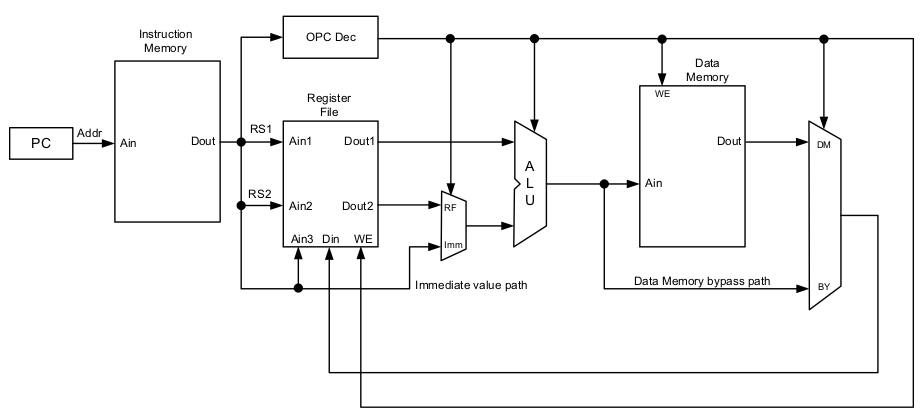
\includegraphics[scale=0.36]{ISA_basic_processor}
%\caption{Basic structure of a \ac{uP}.}
%\label{Figure:basic_registers}
%\end{figure}
%\end{frame}


\end{document}
